\documentclass[border=12pt]{standalone}
\usepackage[utf8]{inputenc}
\usepackage[utf8]{vietnam}
\usepackage{amsmath,amsfonts,amssymb}
\usepackage{tikz}
\usetikzlibrary{arrows, decorations.markings, calc, fadings, decorations.pathreplacing, patterns, decorations.pathmorphing, positioning}

\begin{document}
    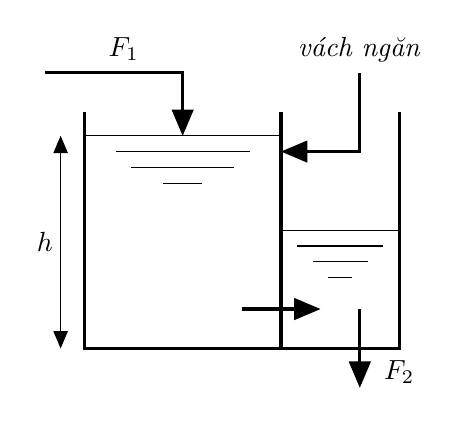
\begin{tikzpicture}[>=triangle 45]
        % Vẽ bình chứa
        \draw[line width=1.2pt] (0,3) -- (0,0) -- (4,0) -- (4,3);
        \draw (0,2.7) -- (2.5,2.7);
        \draw (0.4,2.5) -- (2.1, 2.5);
        \draw (0.6,2.3) -- (1.9, 2.3);
        \draw (1,2.1) -- (1.5, 2.1);
        \draw[line width=1.2pt]  (-.5,3.5) -- (1.27,3.5);

        \draw[line width=1.2pt] (2.5, 3) -- (2.5, 0);
        \draw[line width=1.2pt, <-] (2.5, 2.5) -- (3.52,2.5);
        \draw[line width=1.2pt] (3.5, 2.5) -- (3.5, 3.5);
        \draw (3.5, 3.8) node {$\text{\textit{vách ngăn}}$};
        \draw (2.5,1.5) -- (4, 1.5);
        \draw (2.7,1.3) -- (3.8, 1.3);
        \draw (2.9,1.1) -- (3.6, 1.1);
        \draw (3.1,.9) -- (3.4, .9);

        \draw[line width=1.2pt, ->] (1.25,3.5) -- (1.25,2.7);
        \draw (.5,3.8) node {$F_1$};
        \draw[<->] (-0.3,0) -- (-0.3,2.7);
        \draw (-0.5, 1.35) node {$h$};

        \draw[line width=1.2pt, ->] (2,.5) -- (3,.5);
        \draw[line width=1.2pt, ->] (3.5,.5) -- (3.5,-.5);
        \draw (4, -.3) node {$F_2$};
    \end{tikzpicture}
\end{document}
